\thispagestyle{empty}
\BgThispage
%\begin{flushright}
%    \mbox{потрахаться и сдохнуть потрахаться и сдохнуть потрахаться и сдохнуть потрахаться и сдохнуть потрахаться и сдохнуть потрахаться и сдохнуть потрахаться и сдохнуть }
%\end{flushright}
\begin{flushright}
    \mbox{993 986 979 972 965 958 951 944 937 930 923 916 909 902 895 888 881 874 867 860 853 846 839 832 825 818 811 804 797 790 783 776 769 762 755 748 741 734 727}
\end{flushright}
%\begin{figure}[H]
%    
\includegraphics[scale=0.228]{img/dfsdfa}
%\end{figure}
\vspace{3cm}
\tableofcontents

\newpage

\thispagestyle{empty}

\BgThispage


\section{Задание/}
\begin{enumerate}
    \item Для своей программы из лабораторной работы \#3 по дисциплине \("\)Веб-программирование\("\) реализовать/
    \begin{itemize}
        \item MBean, считающий общее число установленных пользователем точек/ а также число точек, не попадающих в область/ В случае, если пользователь
        совершил 4 "промаха" подряд, разработанный MBean должен отправлять оповещение об этом событии/
        \item MBean, определяющий площадь получившейся фигуры/
    \end{itemize}
    \item С помощью утилиты JConsole провести мониторинг программы/
    \begin{itemize}
        \item Снять показания MBean-классов, разработанных в ходе выполнения задания 1/
        \item Определить имя и версию ОС, под управлением которой работает JVM/
    \end{itemize}
    \item С помощью утилиты VisualVM провести мониторинг и профилирование программы/
    \begin{itemize}
        \item Снять график изменения показаний MBean-классов, разработанных в ходе выполнения задания 1, с течением времени/
        \item Определить имя класса, объекты которого занимают наибольший объём памяти JVM/ определить пользовательский класс, в экземплярах которого
        находятся эти объекты/
    \end{itemize}
    \item С помощью утилиты VisualVM и профилировщика IDE NetBeans/ Eclipse или Idea локализовать и устранить проблемы с производительностью в
    \href{https://se.ifmo.ru/documents/10180/189115/HttpUnit.tar.gz/7bf1032e-d16e-be85-c71b-dbe73c0178ba?t=1651168887037&download=true}{программе}/
    По результатам локализации и устранения проблемы необходимо составить отчёт, в котором должна содержаться следующая информация/
    \begin{itemize}
        \item Описание выявленной проблемы/
        \item Описание путей устранения выявленной проблемы/
        \item Подробное (со скриншотами) описание алгоритма действий, который позволил выявить и локализовать проблему/
    \end{itemize}
\end{enumerate}
Студент должен обеспечить возможность воспроизведения процесса поиска и локализации проблемы по требованию преподавателя/

\newpage

\thispagestyle{empty}

\BgThispage


\section{MBeans/}

\subsection{Исходный код MBean'a, снимающего метрику:}
\tiny
\begin{verbatim}
public class Metrics extends NotificationBroadcasterSupport implements MetricsMXBean, Serializable {

    private int hitsCount = 0;
    private int missedHitsCount = 0;
    private int missedHitsStreakCount = 0;
    int sequenceNumber = 1;

    public Metrics() {
    }

    @Override
    public int hitsInc() {
        hitsCount++;
        return hitsCount;
    }

    @Override
    public int missedAndStreakInc() {
        missedHitsCount++;
        missedHitsStreakCount++;
        if (missedHitsStreakCount % 4 == 0) {
            final Notification notification = new Notification("4 miss streak", this, sequenceNumber++, "4 miss streak.");
            sendNotification(notification);
        }
        return missedHitsStreakCount;
    }

    @Override
    public int clearMissedStreak() {
        missedHitsStreakCount = 0;
        return 0;
    }

    public int getHitsCount() {
        return hitsCount;
    }

    public int getMissedHitsCount() {
        return missedHitsCount;
    }

    public int getMissedHitsStreakCount() {
        return missedHitsStreakCount;
    }

}

\end{verbatim}

\subsection{Исходный код MBean'a, считающего площадь фигуры:}
\begin{verbatim}
public class Square implements SquareMXBean, Serializable {
    double lastSquare = 0;

    public Square() {
    }

    @Override
    public double calculateSquare(double r) {
        double squareSquare = r * 0.5 * r * 1;
        double triangleSquare = (r * (r / 2)) / 2;
        double circleSquare = (Math.PI * r * r) / 4;
        double totalSquare = squareSquare + triangleSquare + circleSquare;
        lastSquare = totalSquare;
        return totalSquare;
    }

    @Override
    public double getLastSquare() {
        return lastSquare;
    }

}

\end{verbatim}

\newpage

\thispagestyle{empty}

\BgThispage

\subsection{Исходный код основного EJB бина приложения, создающего бины и вызывающего их методы:}
\begin{verbatim}
public class AppBean {

    private MBeanServer mbs;
    MetricsMXBean metricsMXBean;
    SquareMXBean squareMXBean;

    public AppBean(List<Result> results) {
        this.mbs = ManagementFactory.getPlatformMBeanServer();
        this.metricsMXBean = new Metrics();
        this.squareMXBean = new Square();
        ObjectName metricsName = null;
        ObjectName squareName = null;
        try {
            metricsName = new ObjectName("AppBean:name=metricsMXBean");
            squareName = new ObjectName("AppBean:name=squareMXBean");
            mbs.registerMBean(metricsMXBean, metricsName);
            mbs.registerMBean(squareMXBean, squareName);
        } catch (Exception e) {
            e.printStackTrace();
        }
    }

    private void resultMBeansHandle(Result result) {
        metricsMXBean.hitsInc();
        if (result.isMatch()) {
            metricsMXBean.clearMissedStreak();
        } else {
            metricsMXBean.missedAndStreakInc();
        }
        double currSquare = squareMXBean.calculateSquare(result.getR());
    }

}
\end{verbatim}

\normalsize

\begin{figure}[H]
    \centering
    
\includegraphics[scale=0.5]{img/trahat}
\end{figure}

\newpage

\thispagestyle{empty}

\BgThispage

\begin{figure}[H]
    \centering
    
\includegraphics[scale=0.5]{img/трахать}
\end{figure}

\newpage

\thispagestyle{empty}

\BgThispage


\section{Мониторинг программы c помощью JConsole/}

\subsection{Показания MBean-классов/}

\subsubsection{Атрибуты MetricsMBean/}
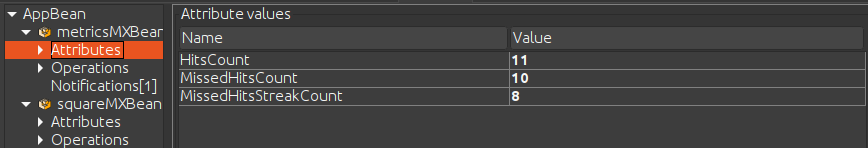
\includegraphics[scale=0.5]{img/Ex2pics/MetricAttributes}

\subsubsection{Операции MetricsMBean/}
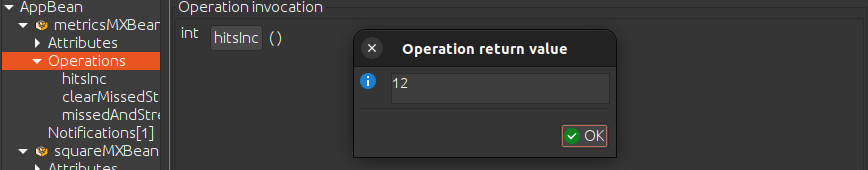
\includegraphics[scale=0.5]{img/Ex2pics/MetricOperations}

\subsubsection{Уведомления MetricsMBean/}
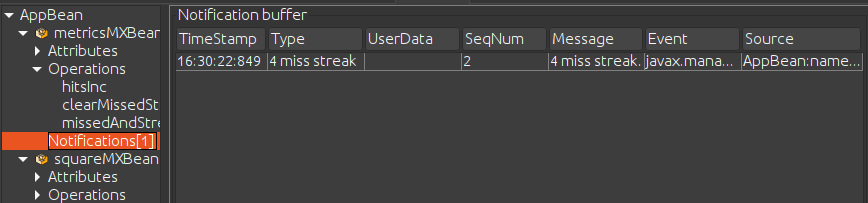
\includegraphics[scale=0.5]{img/Ex2pics/MetricNotif}

\newpage

\thispagestyle{empty}

\BgThispage

\subsubsection{Атрибуты SquareMBean/}
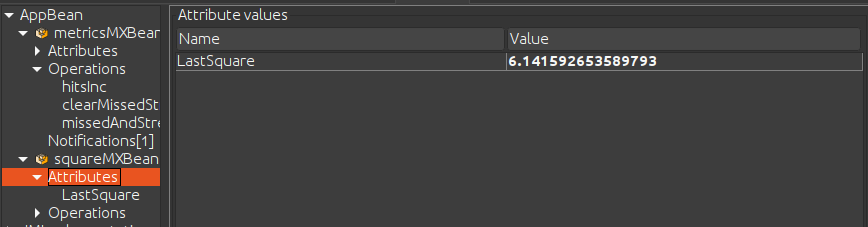
\includegraphics[scale=0.5]{img/Ex2pics/SquareAttributes}

\subsubsection{Операции SquareMBean/}
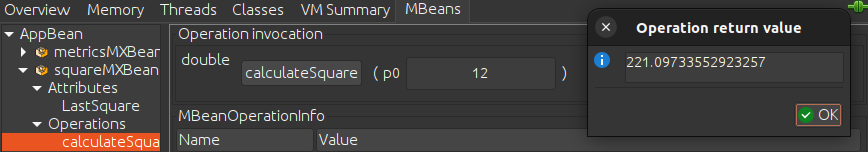
\includegraphics[scale=0.5]{img/Ex2pics/SquareOperations}

\subsection{ОС/}
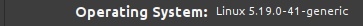
\includegraphics{img/Ex2pics/OS}

\begin{figure}[H]
    \centering
    
\includegraphics[scale=0.4]{img/ghoul}
\end{figure}


\newpage

\thispagestyle{empty}

\BgThispage


\section{Мониторинг и профилирование программы с помощью VisualVM/}

\subsection{Графики изменения показаний MBean-классов/}
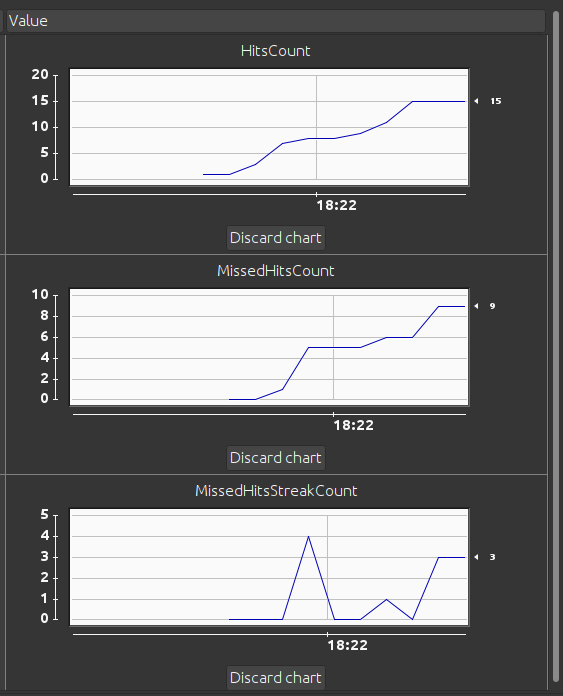
\includegraphics[scale=0.5]{img/Ex3pics/MetricsGraphics}\par
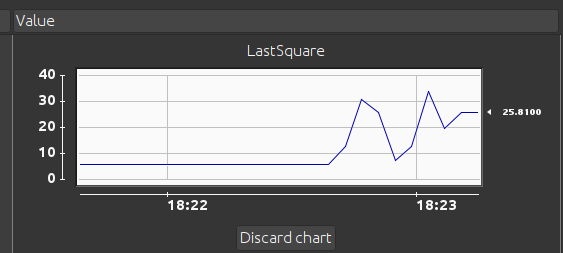
\includegraphics[scale=0.5]{img/Ex3pics/SquareMetrics}

\newpage

\thispagestyle{empty}

\BgThispage

\subsection{Класс, объекты которго занимают наибольший объём памяти/}
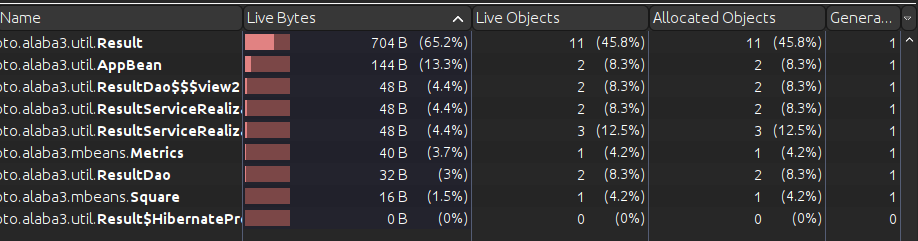
\includegraphics[scale=0.5]{img/Ex3pics/ObjectsMemory}\\
Объекты этого класса хранятся в пользовательском классе AppBean/\par
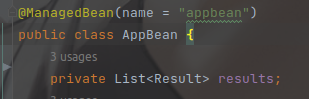
\includegraphics[scale=1]{/home/kyoto/git/report/img/Ex3pics/results}
\vspace{2cm}
\begin{figure}[H]
    
\includegraphics[scale=0.228]{img/dfsdfa}
    
\includegraphics[scale=0.228]{img/dfsdfa}
    
\includegraphics[scale=0.228]{img/dfsdfa}
    
\includegraphics[scale=0.228]{img/dfsdfa}
    
\includegraphics[scale=0.228]{img/dfsdfa}
    
\includegraphics[scale=0.228]{img/dfsdfa}
    
\includegraphics[scale=0.228]{img/dfsdfa}
    
\includegraphics[scale=0.228]{img/dfsdfa}
    
\includegraphics[scale=0.228]{img/dfsdfa}
    
\includegraphics[scale=0.228]{img/dfsdfa}
    
\includegraphics[scale=0.228]{img/dfsdfa}
    
\includegraphics[scale=0.228]{img/dfsdfa}
    
\includegraphics[scale=0.228]{img/dfsdfa}
    
\includegraphics[scale=0.228]{img/dfsdfa}
    
\includegraphics[scale=0.228]{img/dfsdfa}
    
\includegraphics[scale=0.228]{img/dfsdfa}
\end{figure}

\newpage

\thispagestyle{empty}

\BgThispage

\begin{figure}[H]
    \centering
    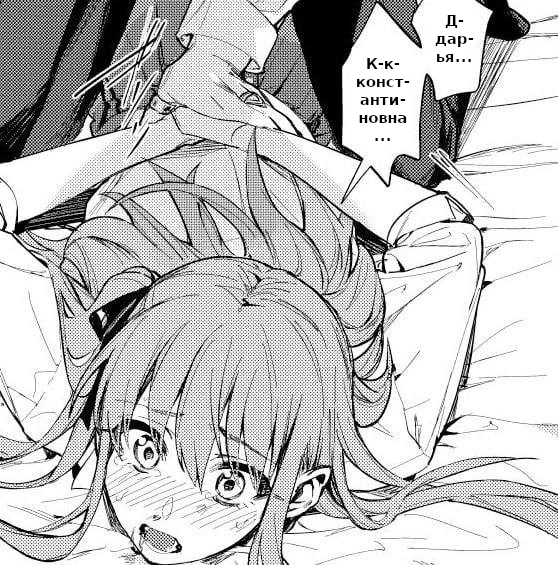
\includegraphics[scale=0.7]{img/rape}
\end{figure}

\newpage

\thispagestyle{empty}

\BgThispage


\section{Локализация и устранение проблемы с производительностью в выданной программе/}

\subsection{Описание выявленной проблемы/}
\begin{enumerate}
    \item "Засыпание" потока на 200мс/
    \begin{figure}[h]
        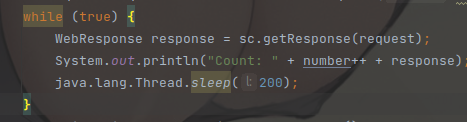
\includegraphics[scale=0.4]{/home/kyoto/git/report/img/Ex4pics/thread.sleep}
    \end{figure}
    \item Отсутствие очищения коллекции сообщений ошибок, в результате чего со временем переполняется память и падает производительность/
\end{enumerate}

\subsection{Пути устранения проблем/}
\begin{enumerate}
    \item Убрать строчку с Thread.sleep()/
    \item 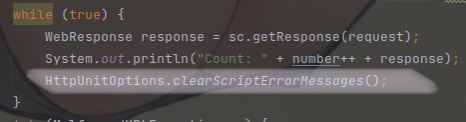
\includegraphics[scale=0.4]{/home/kyoto/git/report/img/Ex4pics/resolved}/
\end{enumerate}

\subsection{Алгоритм выявления проблемы/}
\begin{enumerate}
    \item Воспользуемся методом пристального взгляда на Main-класс, чтобы выявить суть программы - бесконечный цикл с запросами/
    \item Тот же незаменимый метод пристального взгляда позволяет нам заметить/ что после каждого запроса идёт "засыпание" программы на 200мс/ что, несомненно,
    замедляет программу/
    \item Удалим строчку с Thread.sleep() и снизим размер допустимого размера кучи до 30МБайт (установим VM Options "-Xmx30m"), чтобы проблемы обнаружилась
    быстрее, чем я досчитаю 1000-7/
    \item Запустим программу в IDE Idea и откроем график профилировщика и начнём считать/
    \newpage

    \thispagestyle{empty}

    \BgThispage
    
\includegraphics[scale=1.2]{img/993}

    \newpage

    \thispagestyle{empty}

    \BgThispage

    \item Воспользуемся тем же замечательным методом пристального взгляда для обнаружения недопустимого увеличения нагрузки на процессор и сильном
    замедлении программы (примерно 1 запрос в 30 секунд) при приближении размера кучи к установленному максимуму/\\
    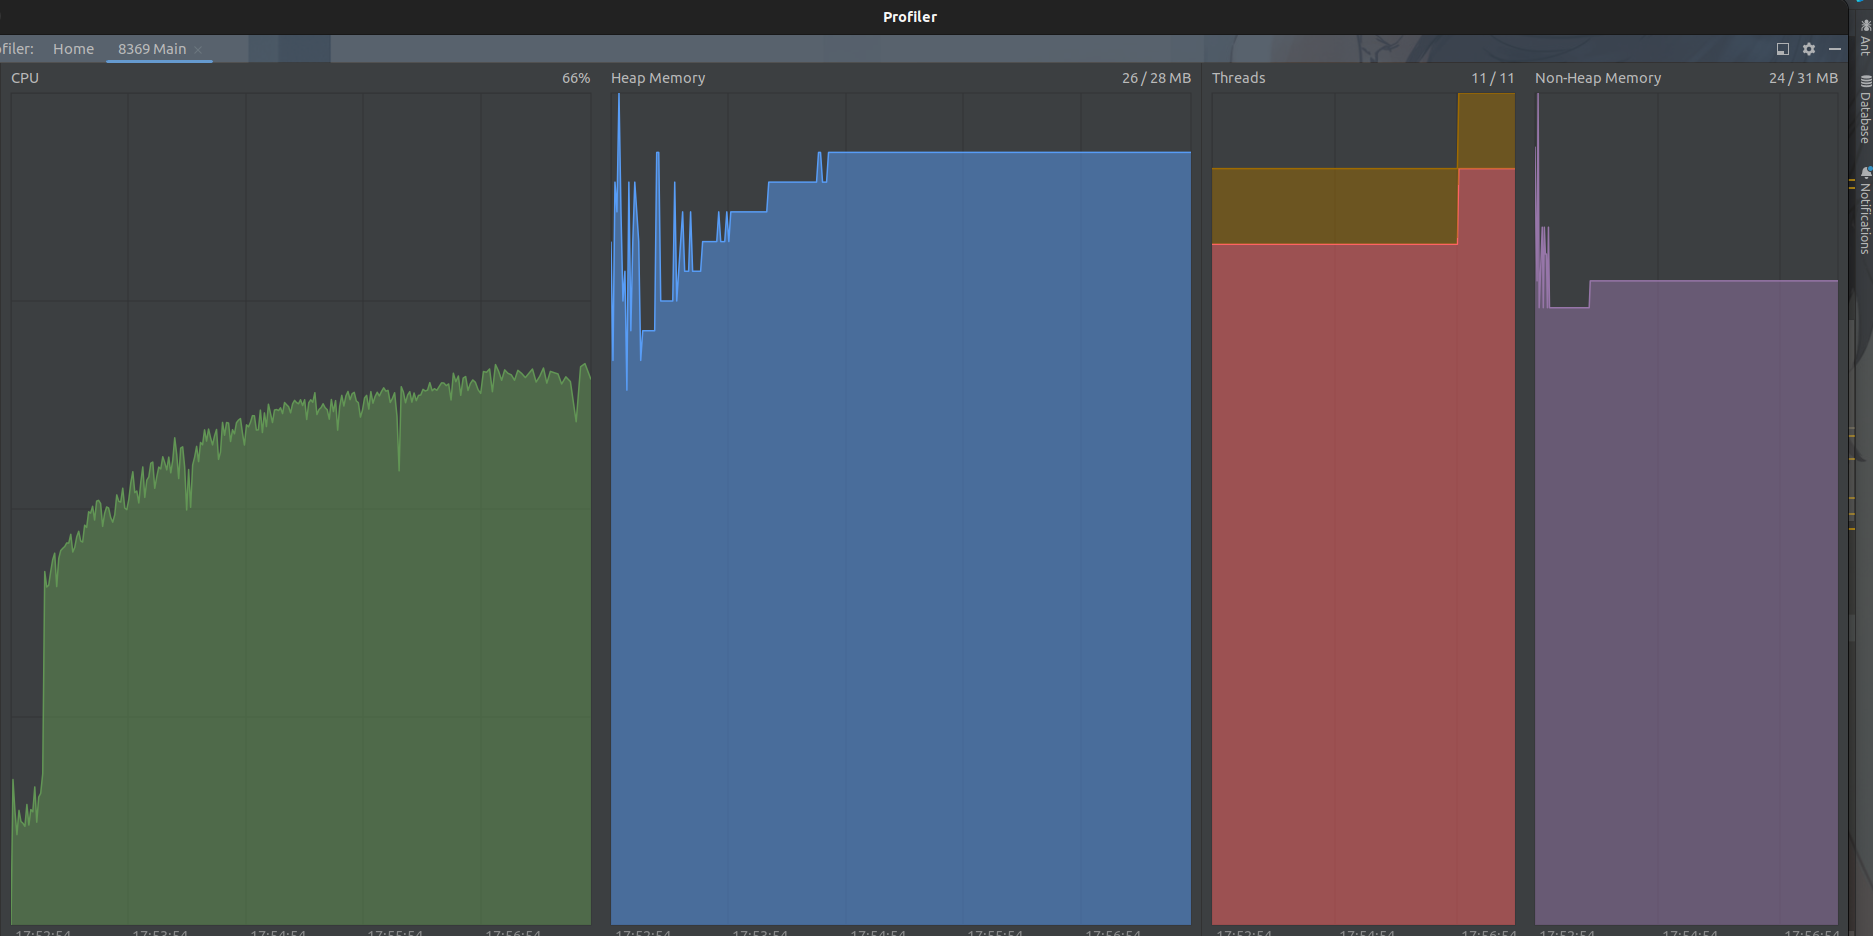
\includegraphics[scale=0.2]{img/Ex4pics/slow_in_IDE}
    \item Запустим программу заново и проанализируем её с помощью VisualVM. Видим там ту же картину/\\
    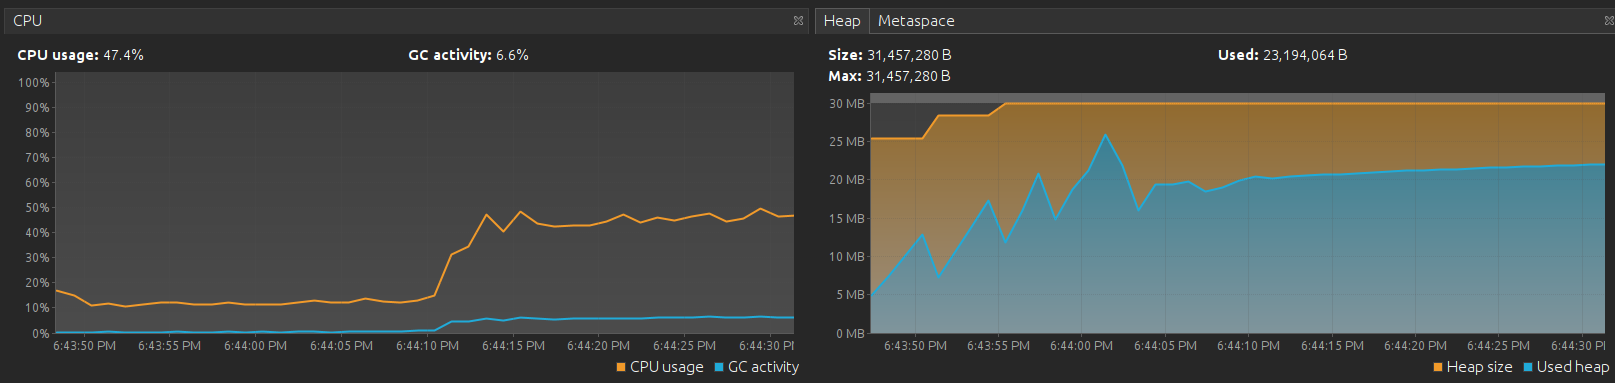
\includegraphics[scale=0.25]{/home/kyoto/git/report/img/Ex4pics/slow_in_visual}
    \item Дополнительно, при мониторинге программы через VisualVM, программа вскоре завершится, выдав OutOfMemoryError/

    \newpage

    \thispagestyle{empty}

    \BgThispage

    \begin{figure}[H]
        \centering
        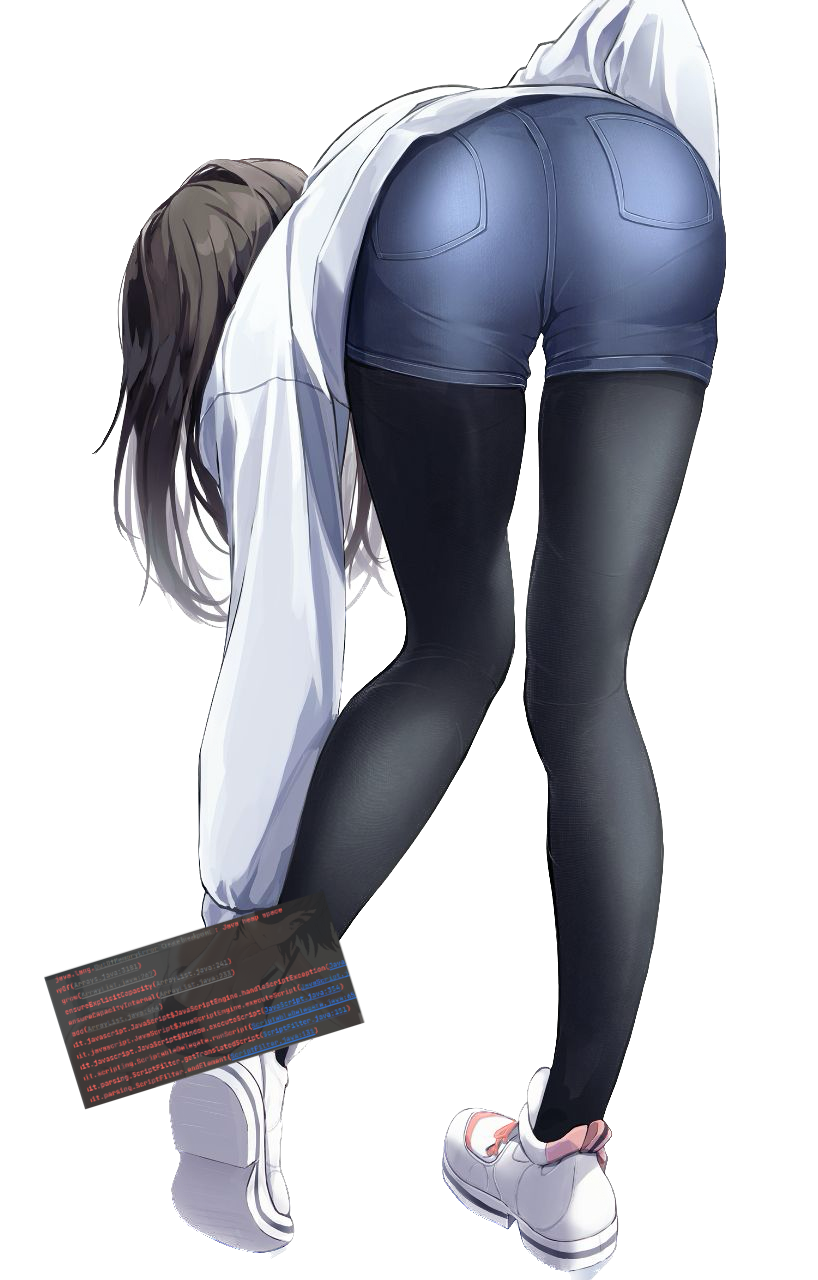
\includegraphics[scale=2]{img/Ex4pics/upala}
    \end{figure}

    \newpage

    \thispagestyle{empty}

    \BgThispage

    \item Создадим Heap Dump и проанализируем объекты в памяти/\\
    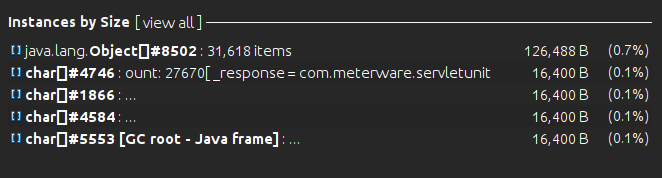
\includegraphics[scale=0.5]{img/Ex4pics/heap_dump}
    \item Нетрудно заметить, какие объекты занимают больше всего места в памяти/\\
    \item Определим, в каком классе они хранятся/\\
    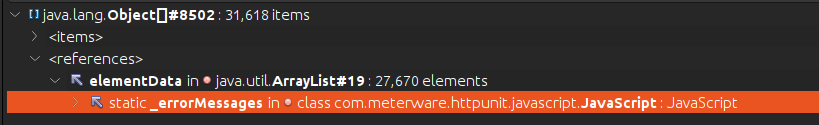
\includegraphics[scale=0.5]{img/Ex4pics/error_messages}
    \item Найдём их в коде и проанализируем/\\
    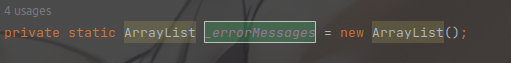
\includegraphics[scale=0.5]{img/Ex4pics/error_messages_in_code}\\
    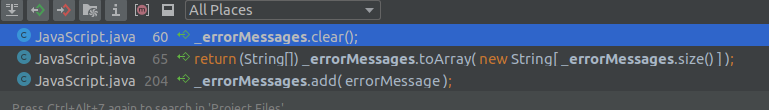
\includegraphics[scale=0.5]{img/Ex4pics/error_messages_usage}
    \item Видим, что на данное поле написан метод, добавляющий ошибки в него, очищающий коллекцию и геттер/
    \newpage

    \thispagestyle{empty}

    \BgThispage

    \item При этом, можно проследить вызовы методов геттера и очищающего/\\
    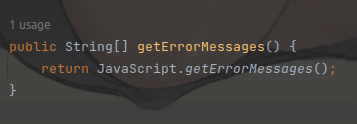
\includegraphics[scale=0.5]{/home/kyoto/git/report/img/Ex4pics/getter1}\\
    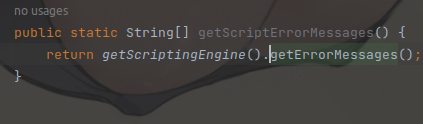
\includegraphics[scale=0.5]{/home/kyoto/git/report/img/Ex4pics/getter2}\\
    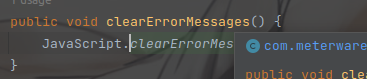
\includegraphics[scale=0.5]{img/Ex4pics/clear1}\\
    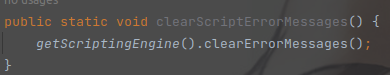
\includegraphics[scale=0.5]{img/Ex4pics/clear2}\\
    \item Нетрудно заметить, что очищающий метод нигде не вызывается/ а так же содержимое данной коллекции нигде в программе не используется/
    \item Будем вызывать метод очистки коллекции после каждого запроса для решения проблемы с переполнением памяти/
    \item Уменьшим размер кучи до 10МБайт промониторим программу через профилировщик IDE Idea/\\
    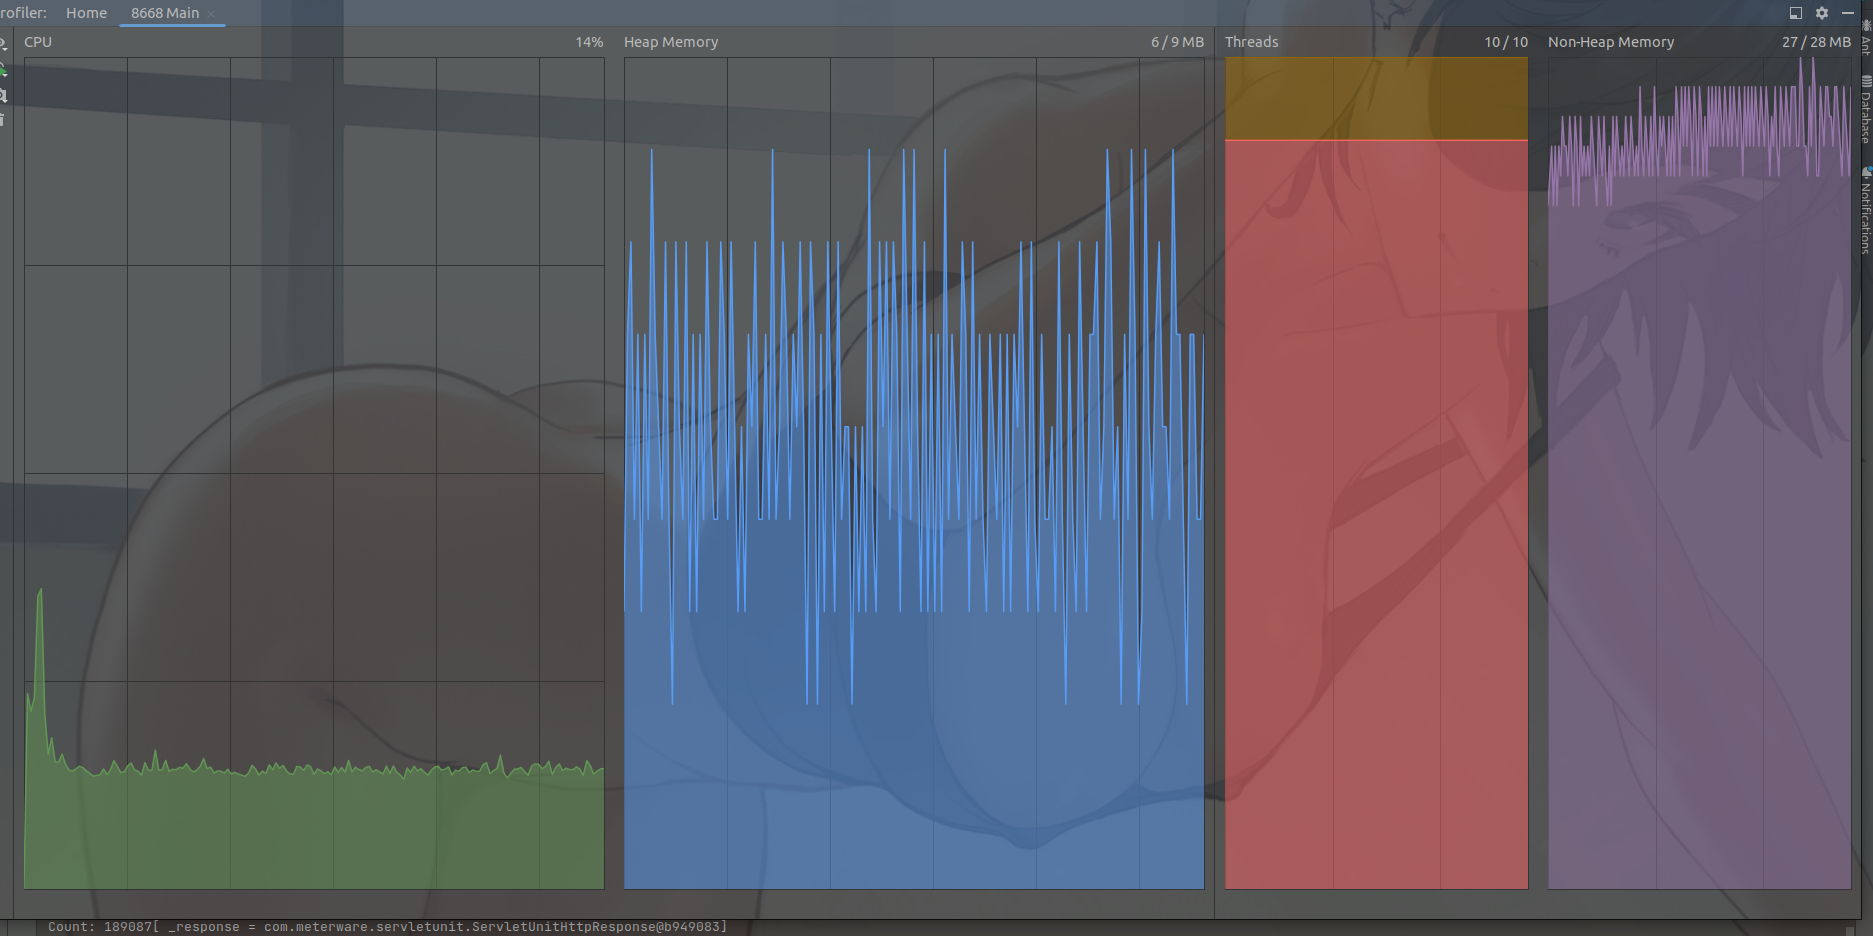
\includegraphics[scale=0.2]{img/Ex4pics/good}

    \newpage

    \thispagestyle{empty}

    \BgThispage

    \item В очередной раз воспользуемся великолепным методом пристального взгляда и увидим, что проблема с производительностью устранена: выделенной памяти
    хватает для корректной работы программы/ а нагрузка на процессор в пределах нормы/
\end{enumerate}


\section{Вывод:}
В ходе программы мы познакомились с MBeans/ утилитами JConsole/ VisualVM и встроенными в IDE профилировщиками/ Можно отметить, что MBeans является
удобной альтернативой дебаггингу для мониторинга работы сложных систем/ а изученные утилиты позволяют подробно проанализировать работу программы и локализовать
возможные ошибки в работе программы и её быстродействии/
\vspace{3cm}
\begin{figure}[H]
    \centering
    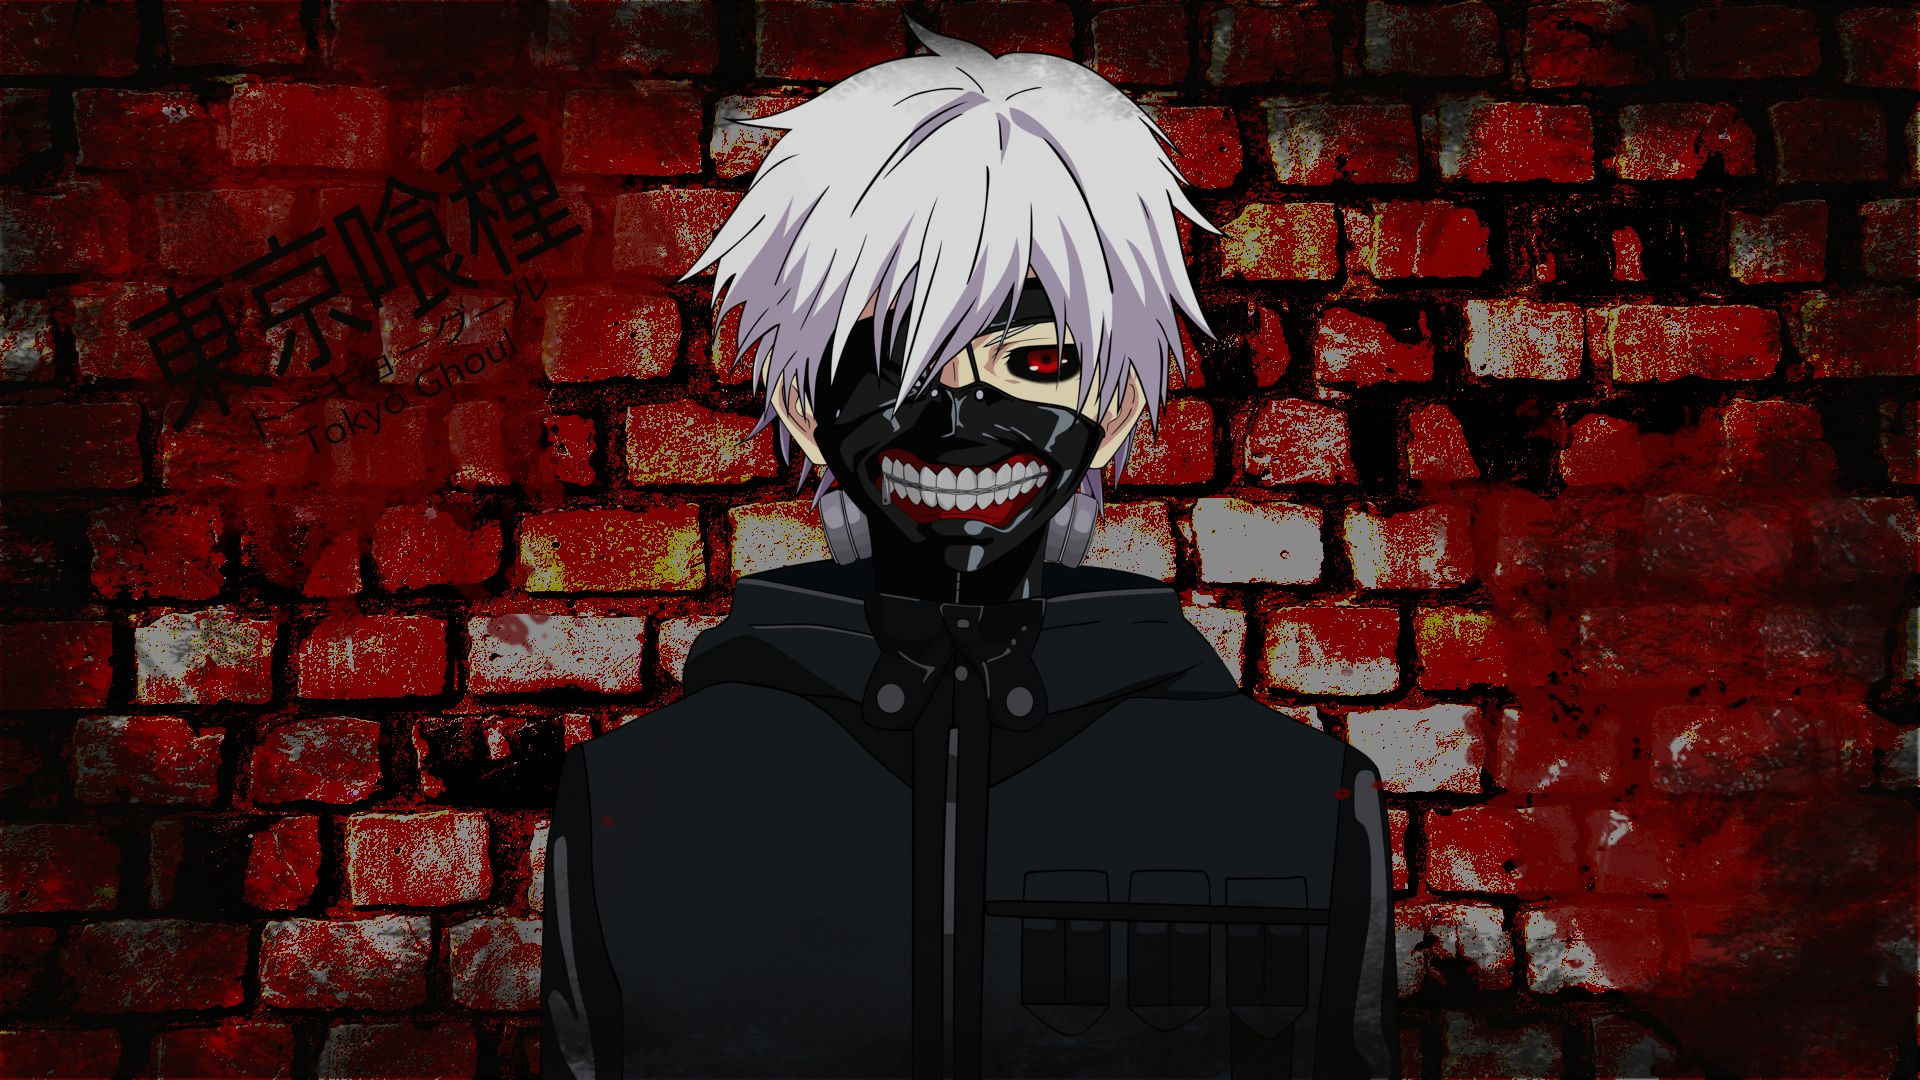
\includegraphics[scale=0.2]{img/39044}
\end{figure}